\documentclass[lang=cn,11pt]{elegantpaper}
\usepackage{booktabs}
\usepackage{multirow}
\usepackage{geometry}
\usepackage{longtable}
\usepackage{pdfpages}


\title{简单GAN模型的训练及其可视化}
\date{}
\begin{document}


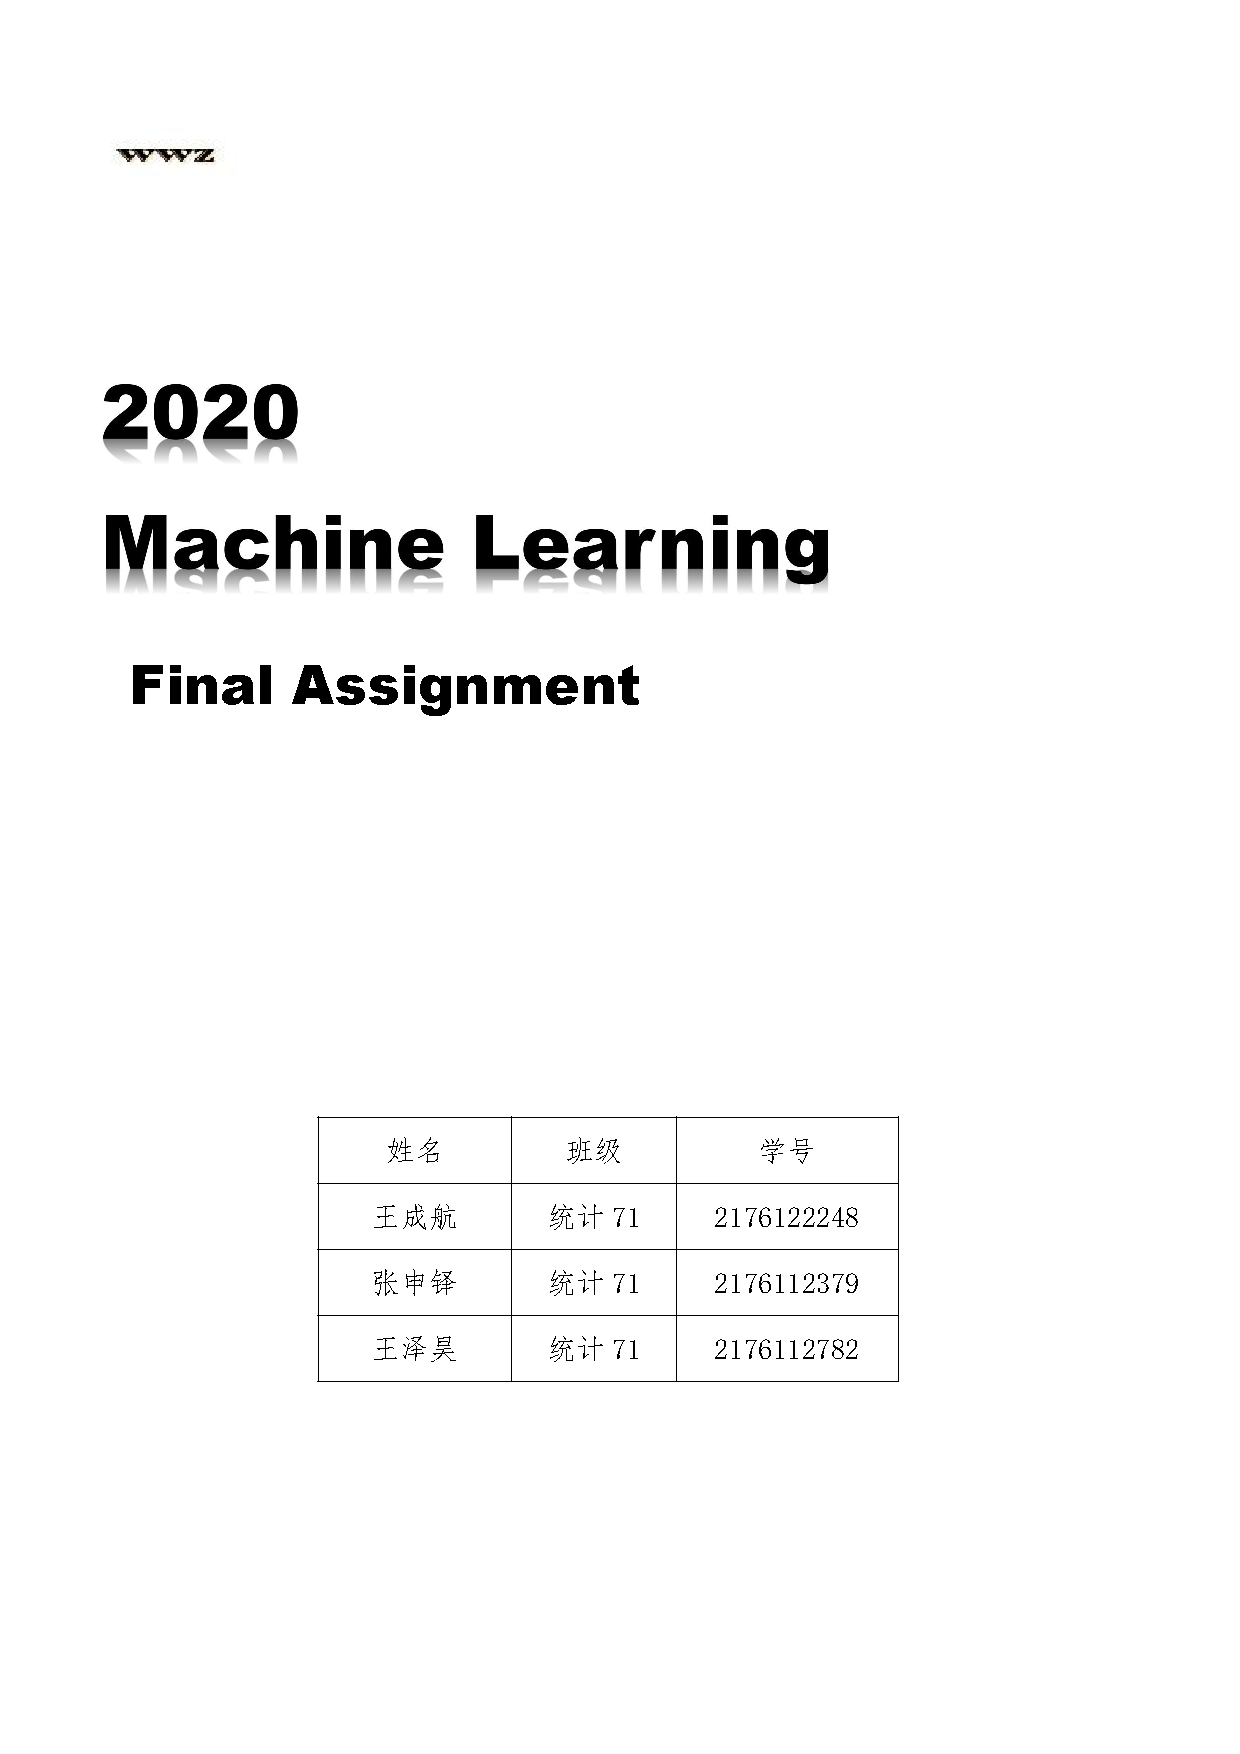
\includepdf[width=\paperwidth]{FM.pdf}
\newpage
\maketitle
\pagenumbering{roman}

\begin{abstract}
本文中, 作者首先通过一个简单的生成式对抗网络生成了与训练样本相类似的狗与飞机的图片, 之后, 又对一些目标是简单的二维图形的GAN训练过程进行了可视化, 并且探究了不同的超参数会对模型的训练产生什么不同的影响. 
\keywords{DCGAN, 可视化, 图像生成}
\end{abstract}
\tableofcontents
\newpage
\pagenumbering{arabic}
\section{GAN简介}

GAN是在2014年由Goodfellow等人提出的一个生成式模型, 它由生成模型G与判别模型D组成. 它可以从随机的噪声分布中生成出一个类似于训练数据的样本, 类似到在统计上无法区分. 

\subsection{工作原理}

GAN的工作原理来源于博弈论中的零和博弈. 其生成模型与判别模型的存在目的都是为了打败对方, 生成模型能够将一个随机向量输出成生成的数据, 而判别模型是以生成或者真实数据为输入, 输出一个标签作为其到底是生成的还是真实的的预测.

生成模型的目标是为了去欺骗判别模型, 随着训练的深入, 生成模型应该能够生成越来越逼真的数据, 以至于判别模型的误判率越来越高. 而判别模型也在不断适应着生成模型, 其对数据真实性的判定标准随着训练的深入也变得越来越高, 因此, 到最后判别模型的判断正确率应保持在$0.5$附近. 

而这样的训练过程一旦结束, 对生成器输入一个噪声, 就可以以一个较高的可信度把这个随机噪声转化成一个统计上与真实数据无异的生成数据. 

\begin{figure}[hb]
    \centering
    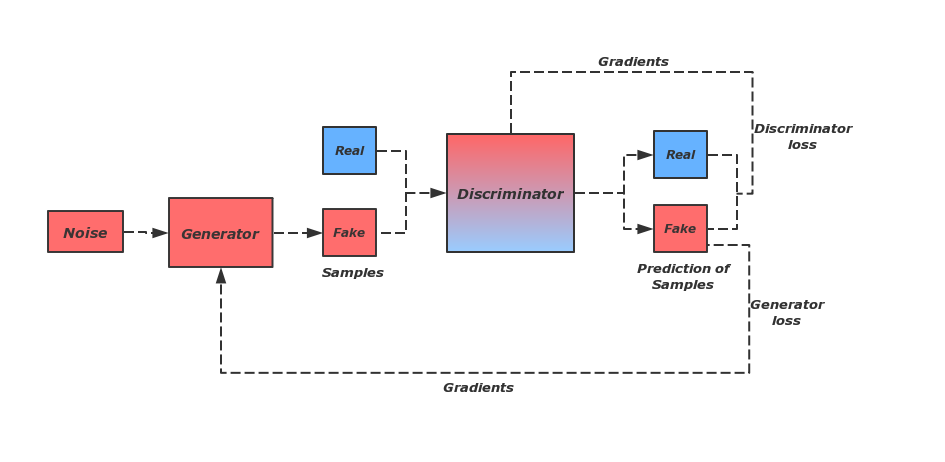
\includegraphics[width=.8\textwidth]{DCGAN}
    \caption{GAN结构示意图. }
\end{figure}

\subsubsection*{生成器}
它将一个向量(噪声)转换为一张图像. 
\subsubsection*{判别器}
它接收一张候选图像(真实的或者生成的)作为输入, 并将其划分到这两个类别之中. 
\subsubsection*{对抗网络}
对抗网络将生成器和判别器连接在一起. 训练时, 这个模型将让生成器向某个方向移动, 从而提高它欺骗判别器的能力. 综合来说, 它将潜在空间的噪声转换为一个分
类决策(真或假). 因此, 训练GAN将会更新生成器的权重, 使得判别器在观察假图像时更有可能预测为“真”. 


\subsection{训练过程}
\begin{enumerate}
  \item 抽取随机噪声
  \item 通过生成模型来生成数据
  \item 将生成数据与真实数据混合并加上标签
  \item 用带标签的数据训练辨别模型
  \item 再一次抽取随机噪声
  \item 再通过生成模型来生成数据
  \item 用刚刚更新过的判别器D所给出的标记为真实数据的标签来更新生成器的权重
\end{enumerate}

\subsection{训练的困难性}

GAN的理论十分美好, 但是GAN的训练十分困难. 对于一个一般的网络, 其优化的最小值通常是固定的. 如果我们用随机梯度下降算法去对性能度量进行优化, 就相当于一个小球在由性能度量所决定的一个地形上滚到最低点. 这个过程是静态的. 

但是对于GAN而言, 整个过程是动态的. 小球每滚一步, 性能度量的地形就会改变一次, 即在GAN中, 我们寻找的不是一个最小值, 而是两个网络之间的一种平衡. 这给训练带来了极大的困难. 它需要我们不断地对各种超参数进行调整, 反复试验从并观察结果. 这也使得GAN的训练成本十分高昂. 目前效果逼真的GAN的每一次训练需要在最先进的单个GPU上跑一个月, 并且每改一次参数我们还需要对网络进行重新训练. 通过这次实验我们深刻地体验到了为什么机器学习被戏称为\textcolor{red}{炼丹术}. 

\section{GAN的简单应用——DCGAN}

我们的尝试是GAN的最典型应用场景, 图像生成. 在此, 我们于 CIFAR10 数据集的图像上来训练 GAN, 主要的原因是它的图像尺寸较小, 模型训练起来可能会轻松一些. 同时, 在训练中, 我们查阅了许多资料, 在这些资料中, 有些作者明确地指出了GAN的某些训练技巧更像是\textcolor{red}{炼金术}而并非科学, 在我们的训练过程中, 这些技巧包括
\begin{itemize}
  \item 使用 tanh 作为生成器最后一层的激活函数, 而不是 sigmoid.
  \item 使用正态分布 (高斯分布) 对潜在空间中的点进行采样, 而不是均匀分布. 
  \item 在训练过程中引入随机性有助于防止GAN“卡住”.
  \item 使用步进卷积代替最大池化来进行下采样, 使用 LeakyReLU 代替 ReLU 激活函数. 
\end{itemize}

\subsection{网络架构}

结合上述的各种启发性技巧, 我们构建了如下的架构作为我们的网络,

\subsubsection*{辨别器}

\begin{figure}[hbt]
\centering
  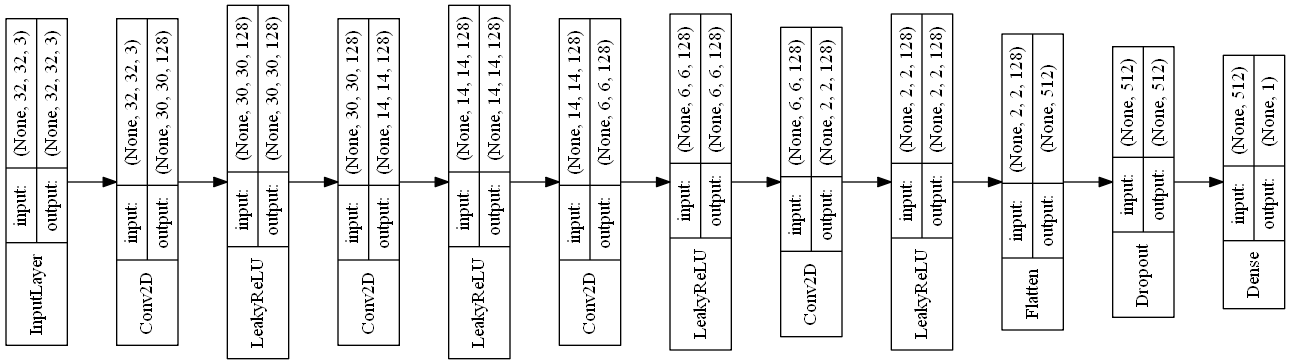
\includegraphics[width=0.95\textwidth]{Arche_D}
  \caption{DCGAN辨别器网络架构}
\end{figure}


\subsubsection*{生成器}

\begin{figure}[hbt]
\centering
  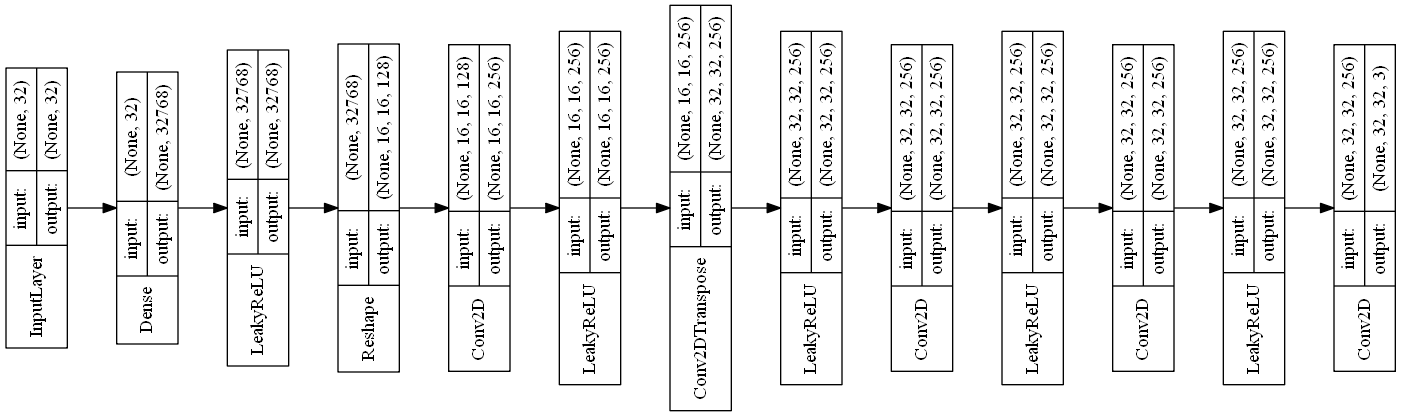
\includegraphics[width=0.95\textwidth]{Arche_G}
  \caption{DCGAN生成器网络架构}
\end{figure}


\subsection{生成图像}
\begin{figure}[htbp]
  \centering
  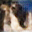
\includegraphics[width=.15\textwidth]{dog1}
  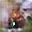
\includegraphics[width=.15\textwidth]{dog2}
  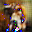
\includegraphics[width=.15\textwidth]{dog3}
  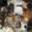
\includegraphics[width=.15\textwidth]{dog4}
  \caption{由GAN生成的狗的图像. \label{fig:dog}}
\end{figure}
在对模型进行少许的调整和训练后, 我们在其众多的结果中挑选出几个较为“漂亮”的图像进行展示. 首先训练生成器生成狗的图像, 如 \figref{fig:dog}, 可以看到, 虽然清晰度并不是十分的高, 而且有的图像上甚至有噪点, 但仍能从大致轮廓以及五官上判断出来是狗的模样. 同样的, 我们还让生成器生成了飞机的图像, 如 \figref{fig:air}, 对于飞机图像的生成似乎比狗的要成功一些, 甚至将机翼, 机身, 尾翼等特征都清晰地表现了出来. 
\begin{figure}[htbp]
  \centering
  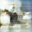
\includegraphics[width=.15\textwidth]{air1}
  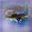
\includegraphics[width=.15\textwidth]{air2}
  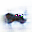
\includegraphics[width=.15\textwidth]{air3}
  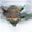
\includegraphics[width=.15\textwidth]{air4}
  \caption{由GAN生成的飞机的图像. \label{fig:air}}
\end{figure}

但总体而言, 由于我们对于超参数的调整有限, 网络结构可能也并不是最优, 训练出来的图像并没有达到以假乱真的地步. 同时, 由于训练GAN生成真实图片的花销也比较大, 因此我们接下来将目标转一些特殊函数的图像. 
\section{GAN的训练过程可视化}

GAN通常都会应用在如生成各种各样的图像的问题上. 这些问题都是十分高维的问题. 假如说要生成$100\times 100$大小的手写数字, 那么输入空间的维度便是$100^2$. 这么高的维度给可视化带来了巨大的困难. 

因此, 我们考虑了一个更加简单的问题. 即对于一个二维均匀分布噪声$\varepsilon \sim \mathrm{Unif}[-1,1]^2$, 给定一个变换$f:\mathbb [-1,1]^2 \to \mathbb [-1,1]^2$, 构造出另外一个概率分布$\mathcal U$. 然后通过GAN来生成$\mathcal U$, 希望生成器能够替代这样的一个函数$f$, 通过均匀分布生成出经过变换构造出的分布$\mathcal U$.

\begin{figure}[htbp]
    \centering
    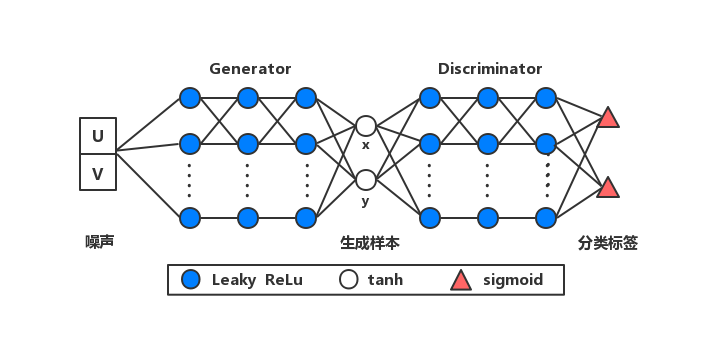
\includegraphics[width=0.6\textwidth]{流程}
    \caption{网络结构示意图. \label{fig:f3}}
\end{figure}


同时, 我们还在GAN训练完每个Batch之后将其可视化. 生成器和判别器的网络都具有三层全连接层, 使用Leaky ReLu激活. 生成器的的学习率为0.0001, 判别器的学习率为0.001, 优化算法都使用参数$\beta=0.5$下的Adam优化器. 网络架构如 \figref{fig:f3} 所示. 在此网络上的训练结果如 \figref{fig:f1} 所示. 
\begin{figure}[htbp]
  \centering
    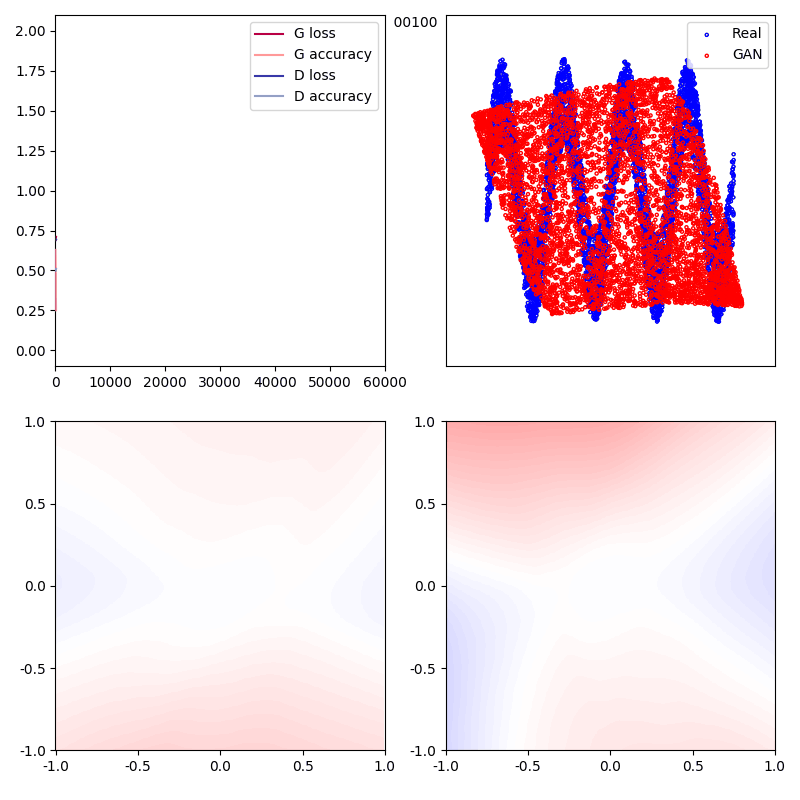
\includegraphics[width=0.35\textwidth]{sin_2_1}
    \caption{训练过程可视化的样图. \label{fig:f1}}
  \end{figure}

\begin{enumerate}
	\item 左上方可以看到每个训练步骤的生成器和判别器的损失 (二进制交叉熵) 和精度.
	\item 右上方为真实样本和伪造样本, 在每个训练步骤之后, 绘制真实分布 (蓝色) 和生成的分布 (红色).
	\item 左下方显示了隐空间中每个点的判别器输出, 其中蓝色表示判别器认为是“绝对是真的”, 红色表示判别器认为是“绝对是假的”, 而白色表示判别器不知道该将其归为哪一类. 
	\item 右下方图与左下方的图非常相似, 不同之处在于它可视化的是样本空间而不是隐空间. 
\end{enumerate}

\subsection{正弦波}

第一个实验是将整个方块变换为正弦波, 即
\begin{align*}
	f_x(x,y)=x,\ f_y(x,y)=sin(x)+\dfrac{y}{4}.
\end{align*}

\begin{figure}[hbt]
\centering
  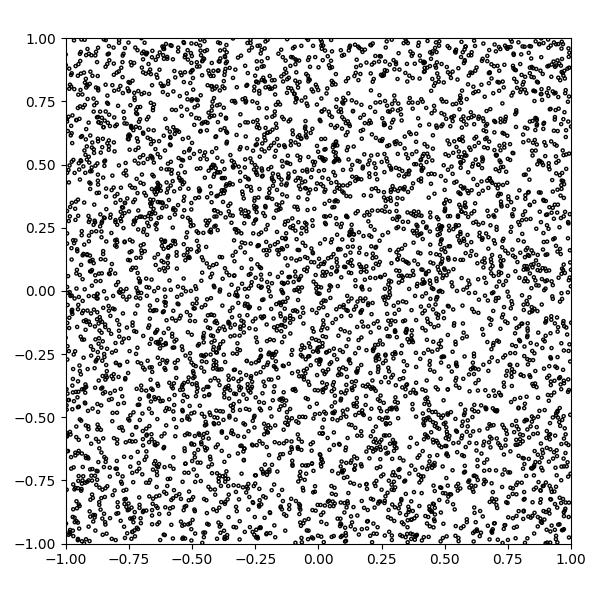
\includegraphics[width=0.2\textwidth]{sin_1_1}  
  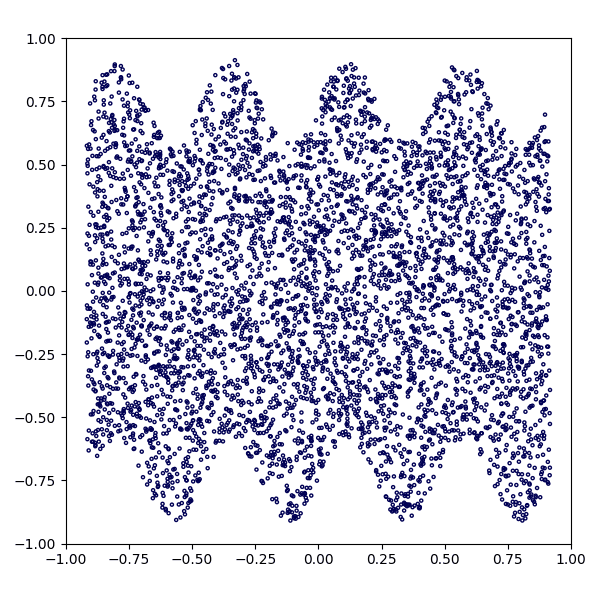
\includegraphics[width=0.2\textwidth]{sin_1_2}
  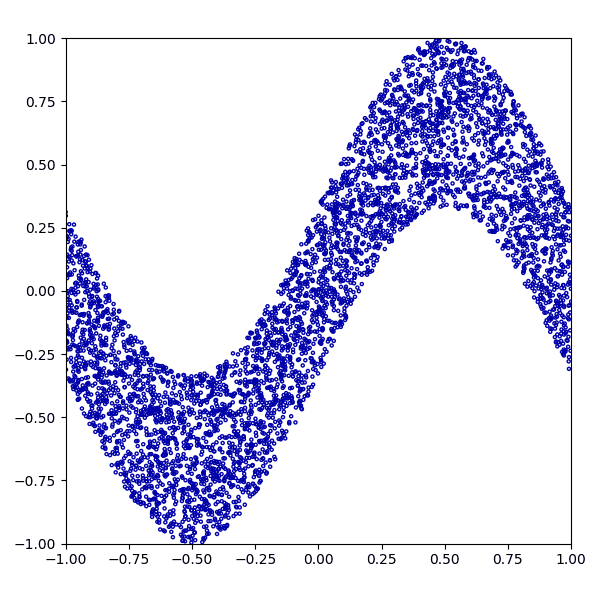
\includegraphics[width=0.2\textwidth]{sin_1_3}
  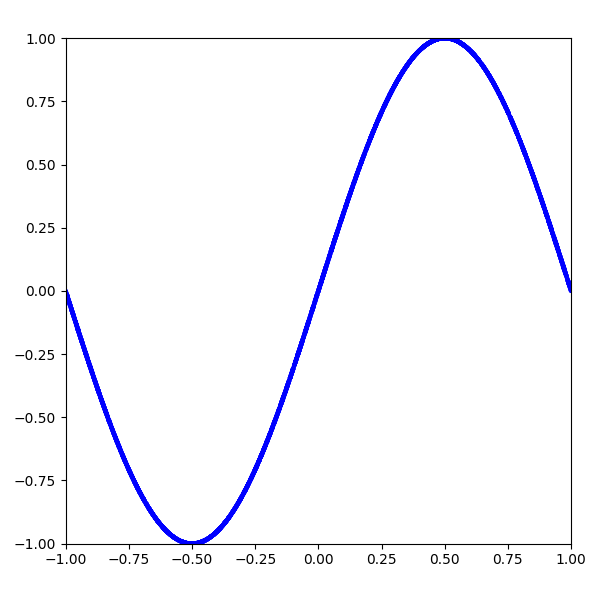
\includegraphics[width=0.2\textwidth]{sin_1_4}
  \caption{从左到右可以看出变换$f$如何从Unif$[-1,1]^2$生成所需分布$\mathcal U$.}
\end{figure}

\noindent 变换后的分布是在正弦波形区域里的均匀分布, 通过实验, 我们发现训练大致可以分为三个时期. 即捕捉大致范围, 捕捉细致分布到最后病态化.

\subsubsection{捕捉大致范围}
在GAN得训练的初期阶段, 判别器在帮助生成器去捕捉分布的大概范围. 并且生成器很快就捕捉到了大致的范围, 这可能是因为函数比较简单.

\begin{figure}[htbp]
\centering
  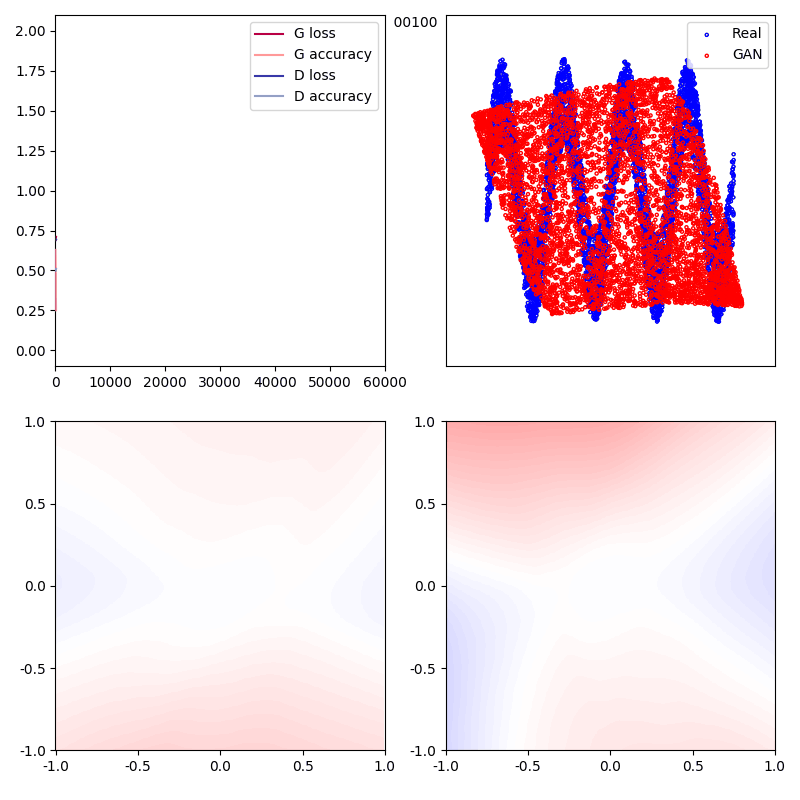
\includegraphics[width=0.35\textwidth]{sin_2_1}
  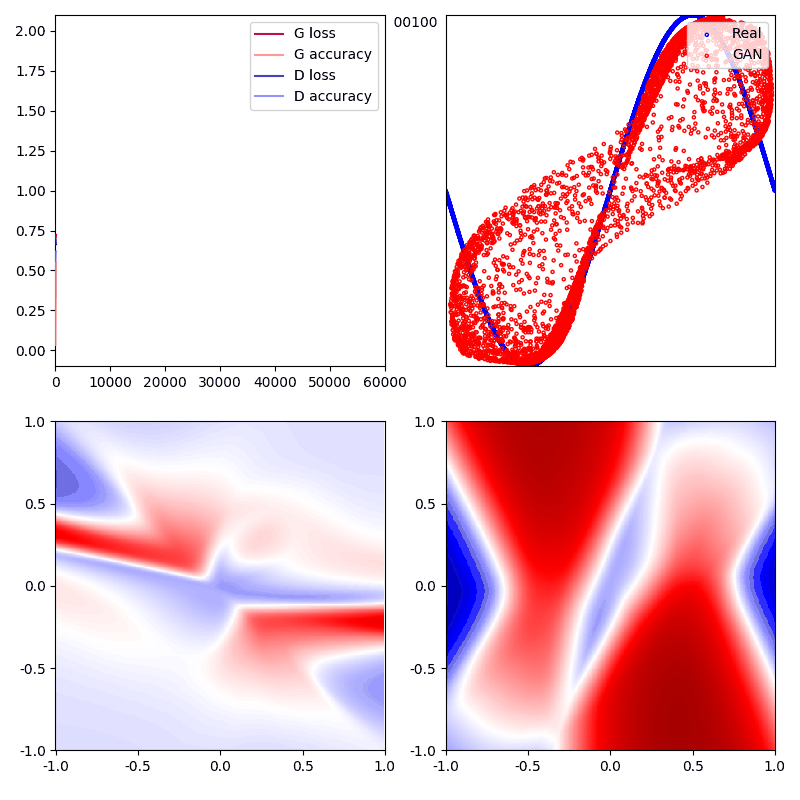
\includegraphics[width=0.35\textwidth]{sin_2_2}
  \caption{捕捉大致范围.}
\end{figure}

\subsubsection{捕捉分布细节}

随着训练的进行, 我们发现在捕捉到大致范围了以后, 生成器生成的点反而相对集中在两个波峰之间的白色区域里, 也就是没有生成出期望的样本. 但随着训练的深入, 判别器成功地帮我们的生成器纠正了这些错误. 在经过15000次训练了以后, 生成器的表现已经很不错了. 只有少部分点落在了白色区域, 大部分点都集中在了真实样本所在的区域. 这个时候可以说生成器已经可以代替$f$来进行数据生成的工作了. 
\begin{figure}[htbp]
\centering
  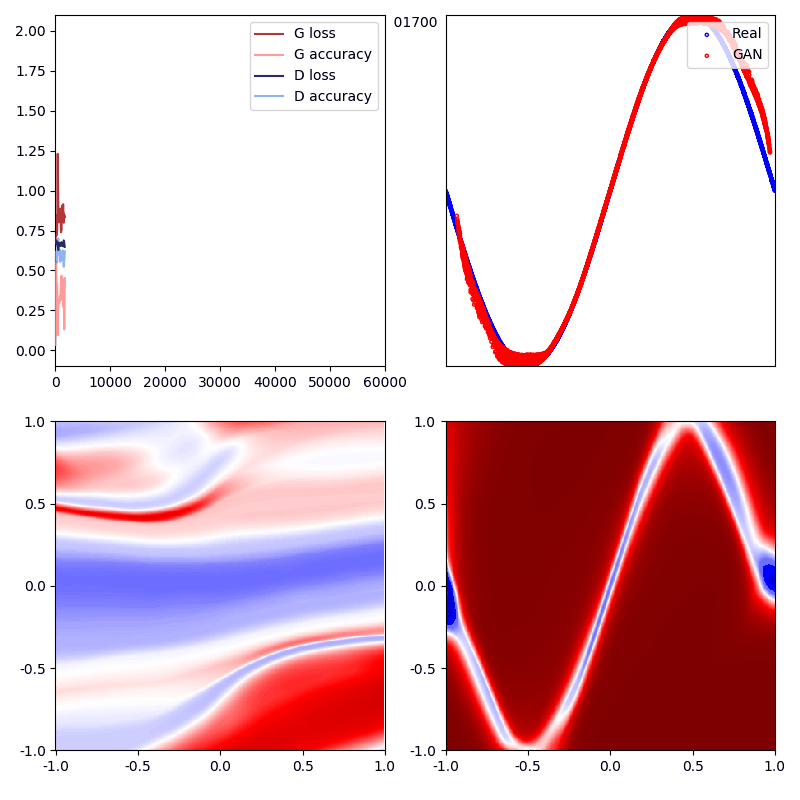
\includegraphics[width=0.3\textwidth]{sin_3_1}
  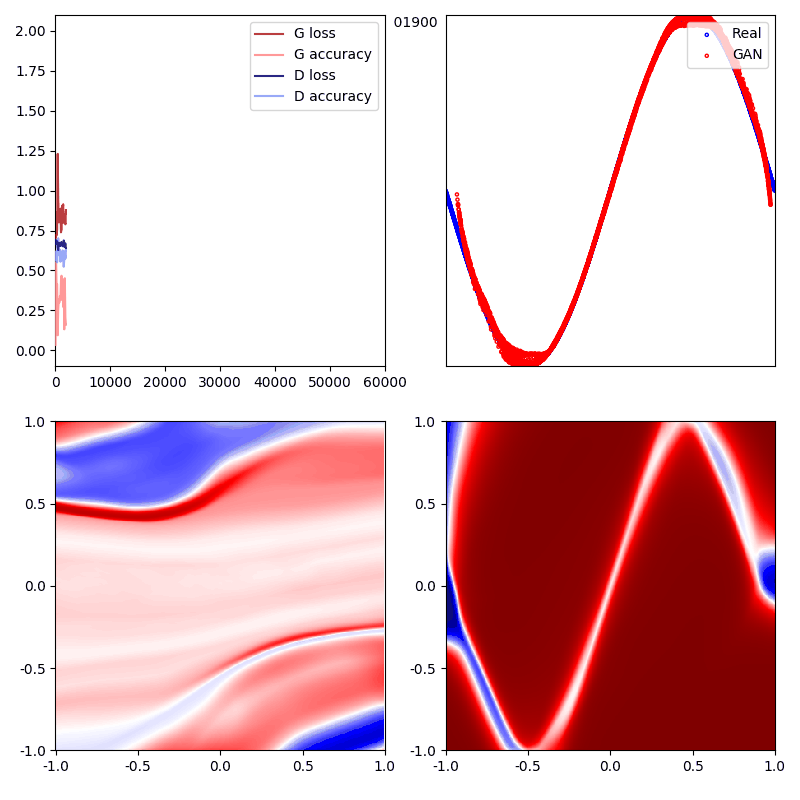
\includegraphics[width=0.3\textwidth]{sin_3_2}\\
  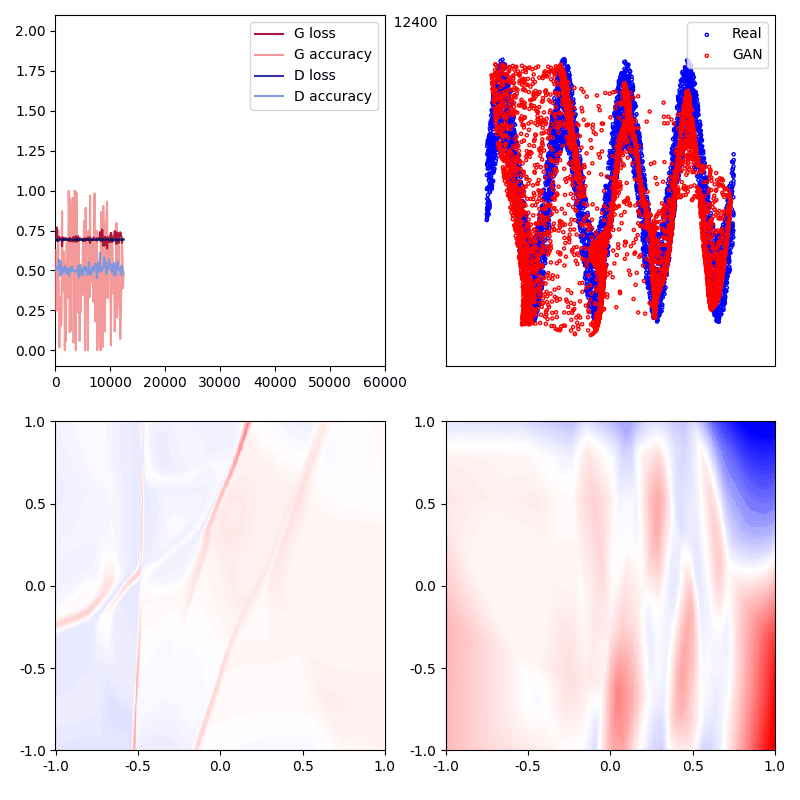
\includegraphics[width=0.3\textwidth]{sin_3_3}
  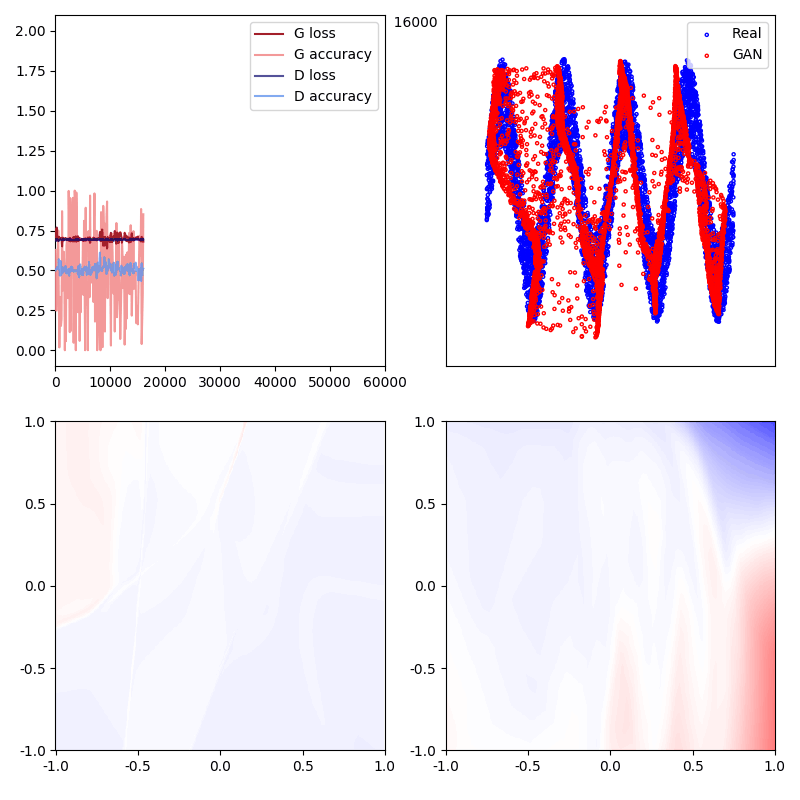
\includegraphics[width=0.3\textwidth]{sin_3_4}
  \caption{捕捉分布细节}
\end{figure}

并且可以看到, 此时的判别器也大致出现了正弦波样式的分类边界, 这似乎意味着我们得判别器应该是要继续执导生成器使得生成器在白色区域的生成样本越来越少. 但是事情并没有朝着我们的预期发展. 

%并且随着训练的进行, 我们的判别器捕捉到的在样本空间中的分类边界反而变得比一开始更加模糊, 之前认为是真实样本的区域完全消失掉了. 原来样本空间中正弦波样式的分类边界逐渐消失变为了一整个判别器无法确定真假的长方形区域. 并且我们在输入空间中的判别器输出大部分都变为了不确定. 同时生成器也出现了较大的波动. 

\subsubsection{病态化}

如 \figref{fig:f2}, 随着训练的深入, 我们发现GAN似乎陷入了一个无法跳出的怪圈. 即判别器指导生成器向着一个错误的方向进行了改进, 并且直到60000次训练结束的时候还是看不到任何的改善. 并且这样的问题从纸面上的性能度量Loss跟Accuracy上面是看不出来的.
\begin{figure}[htbp]
  \centering
  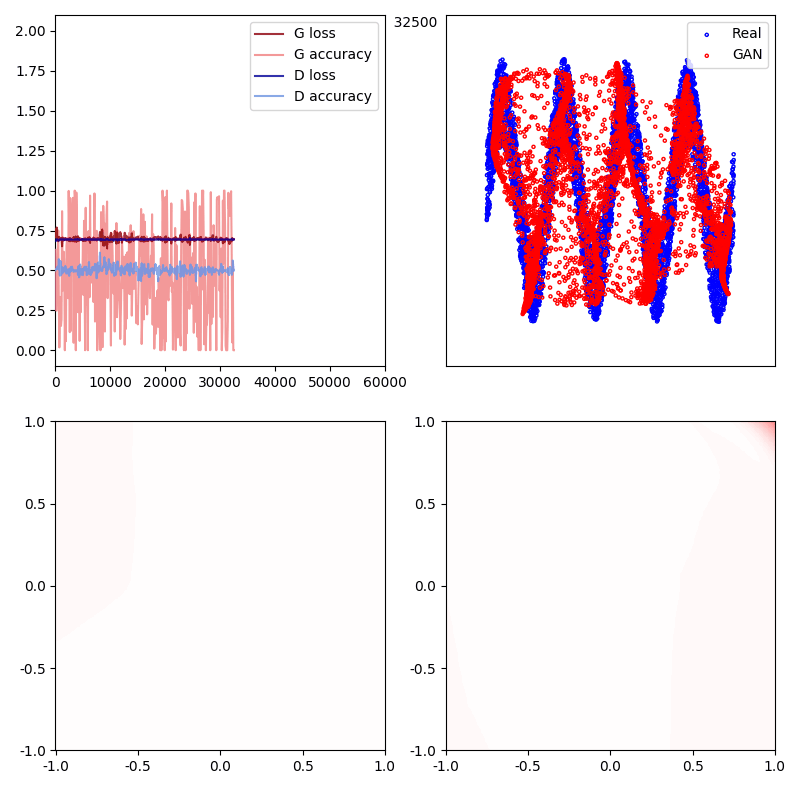
\includegraphics[width=0.3\textwidth]{sin_4_1}
  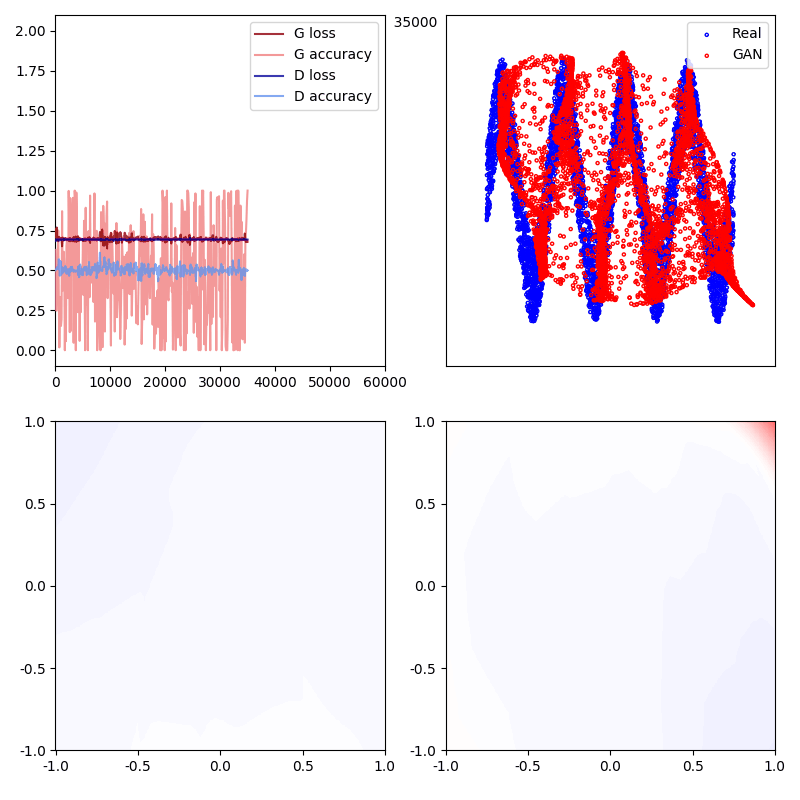
\includegraphics[width=0.3\textwidth]{sin_4_2}
  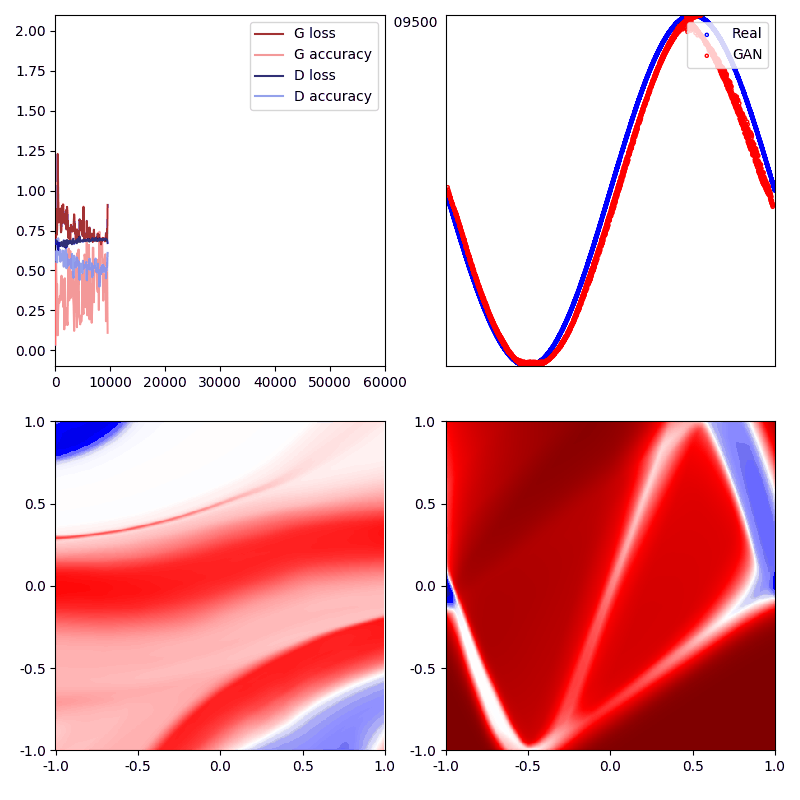
\includegraphics[width=0.3\textwidth]{sin_4_3}\\
  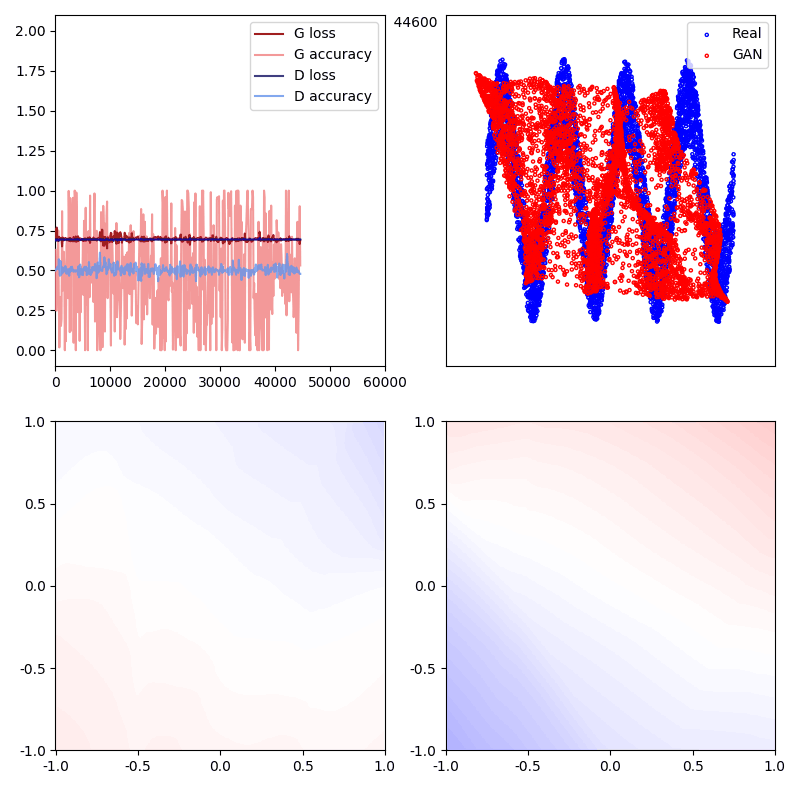
\includegraphics[width=0.3\textwidth]{sin_4_4}
  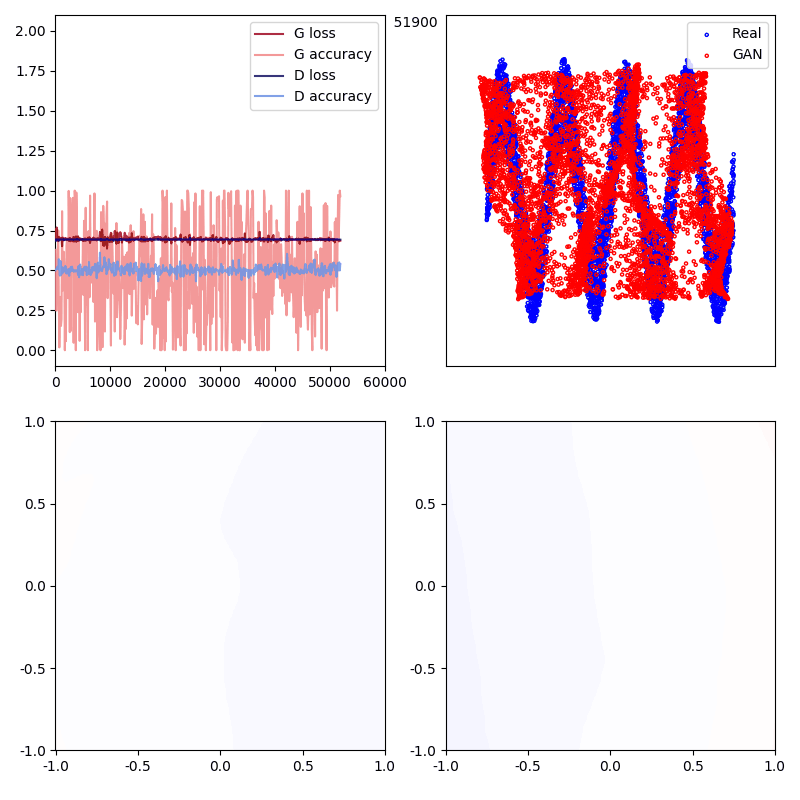
\includegraphics[width=0.3\textwidth]{sin_4_5}
  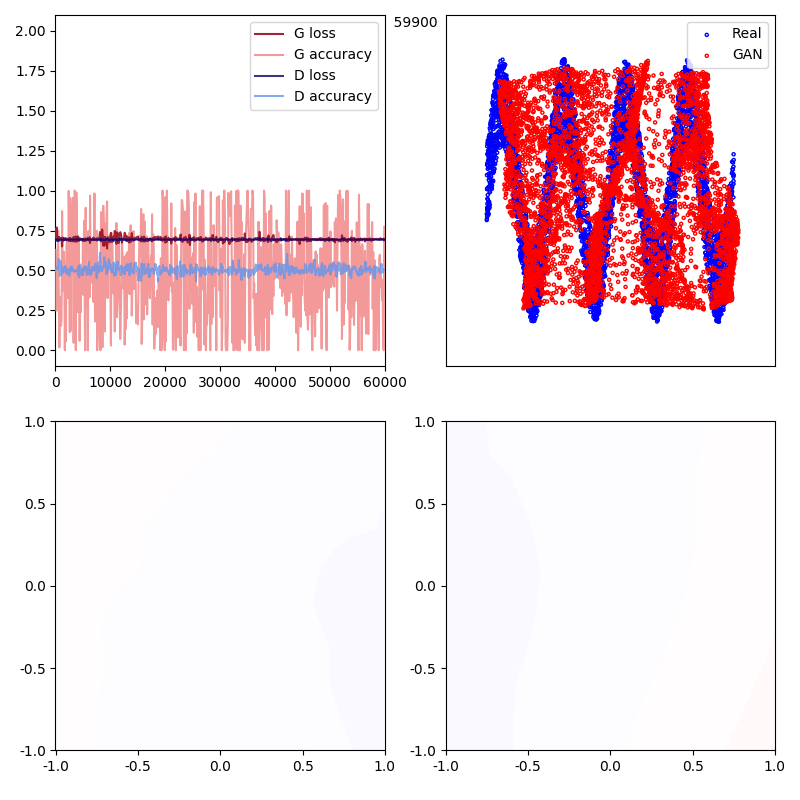
\includegraphics[width=0.3\textwidth]{sin_4_6}
  \caption{病态化. \label{fig:f2}}
\end{figure}

首先在白色区域的生成样本逐渐变多. 逐渐回到了刚刚捕捉到大范围时的状态. 并且可以很明显的看到生成器还因为未知的原因在一条对角线上集中地在生成数据, 我们怀疑我们的训练陷入了一个局部极小值的状态. 此时判别器对生成器没有办法进行有效的指导. 我们猜测这样的现象有如下几种可能

\begin{enumerate}
	\item 网络太浅, 表达能力不足.
	\item 训练次数不够.
	\item 超参不合适.
\end{enumerate}

\noindent 我们通过进一步的实验证实了最有可能是因为超参数的设置不合理. 进一步实验的细节见下文. 




\subsection{圆}
第二个实验是将整个方块变为一个半径为1的圆, 即
\begin{align*}
	f_x(x,y)=\frac{x}{2},\ f_y(x,y)=y\cdot\pi.
\end{align*}
可以证明, 这样变换得到的分布并不是在这个圆上的一个均匀分布. 从图上也可以看出这样的分布下, 数据更有可能处于中心而不是圆的边缘. 
\begin{figure}[htbp]
  \centering
  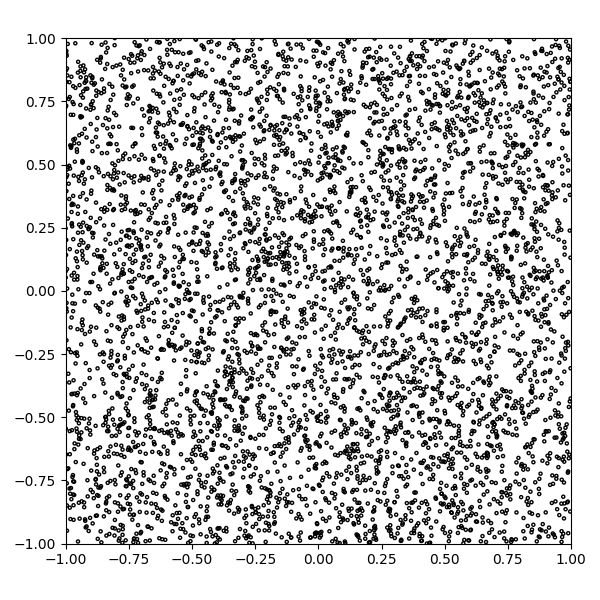
\includegraphics[width=0.1\textwidth]{circle_1_1}
  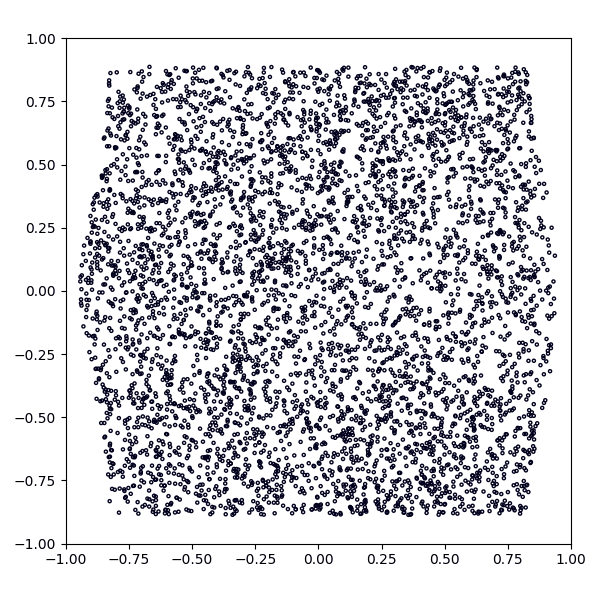
\includegraphics[width=0.1\textwidth]{circle_1_2}
  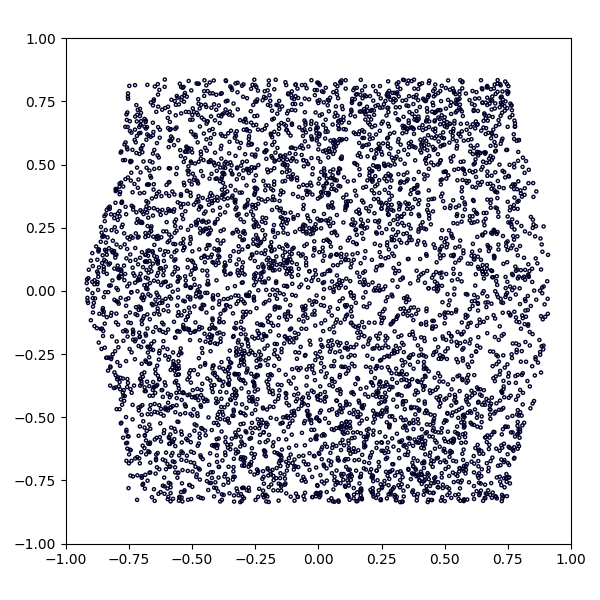
\includegraphics[width=0.1\textwidth]{circle_1_3}
  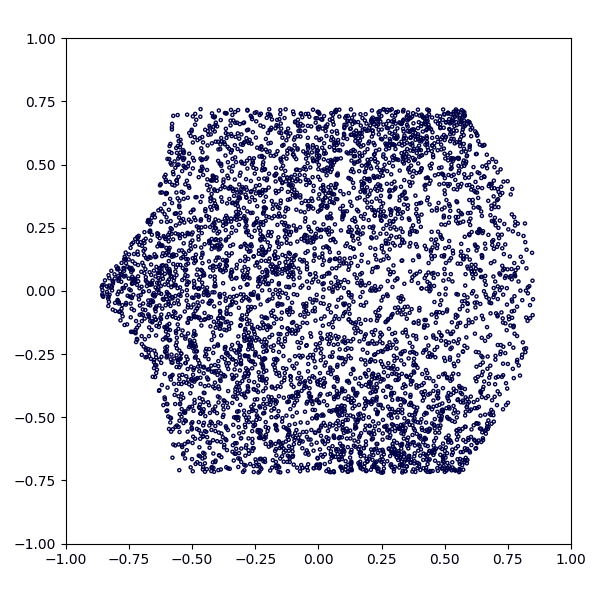
\includegraphics[width=0.1\textwidth]{circle_1_4}
  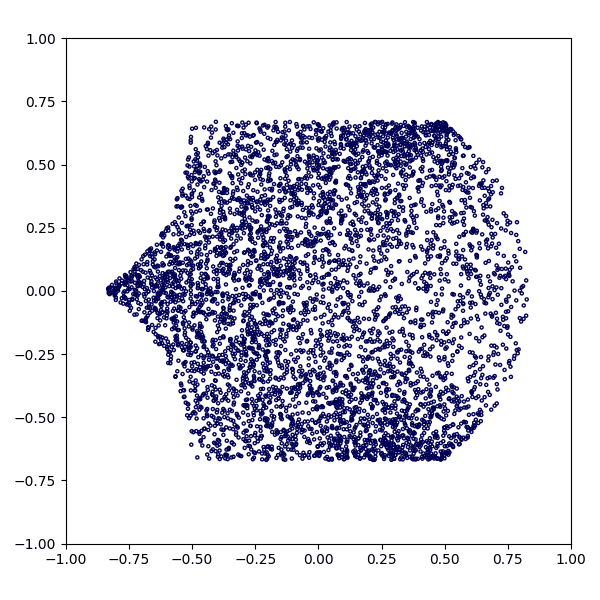
\includegraphics[width=0.1\textwidth]{circle_1_5}
  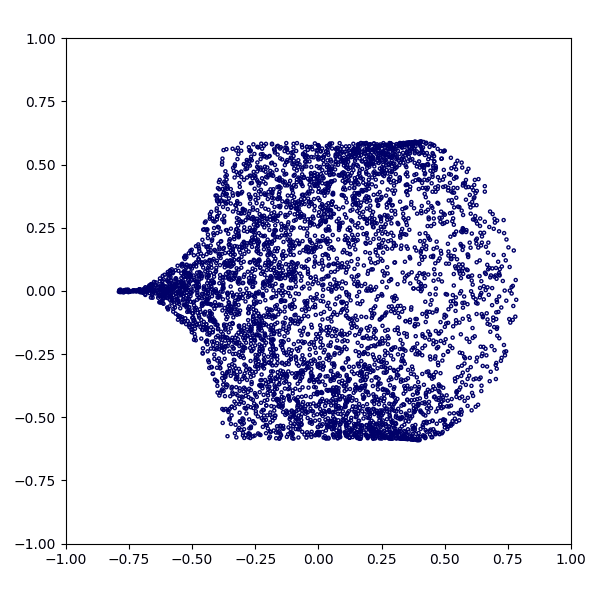
\includegraphics[width=0.1\textwidth]{circle_1_6}\\
  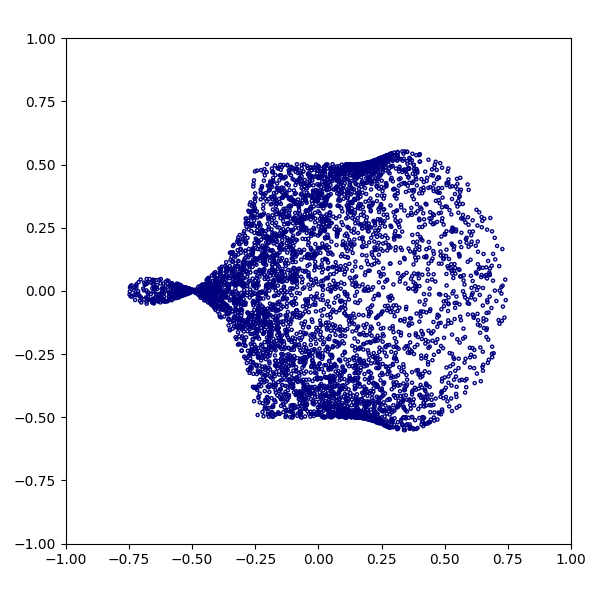
\includegraphics[width=0.1\textwidth]{circle_1_7}
  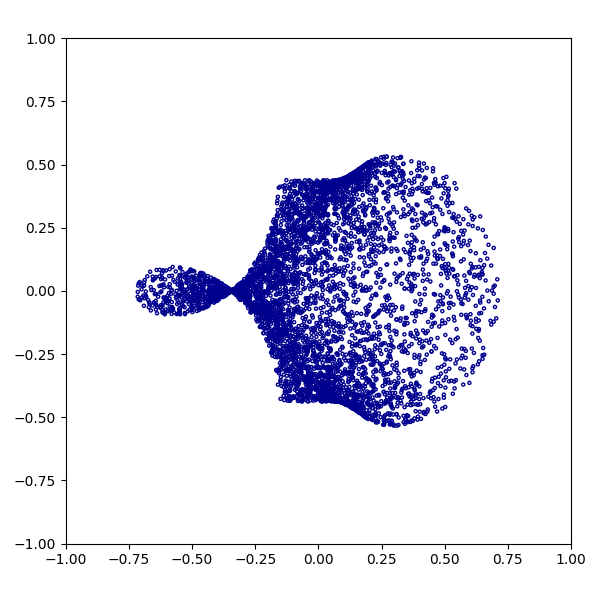
\includegraphics[width=0.1\textwidth]{circle_1_71}
  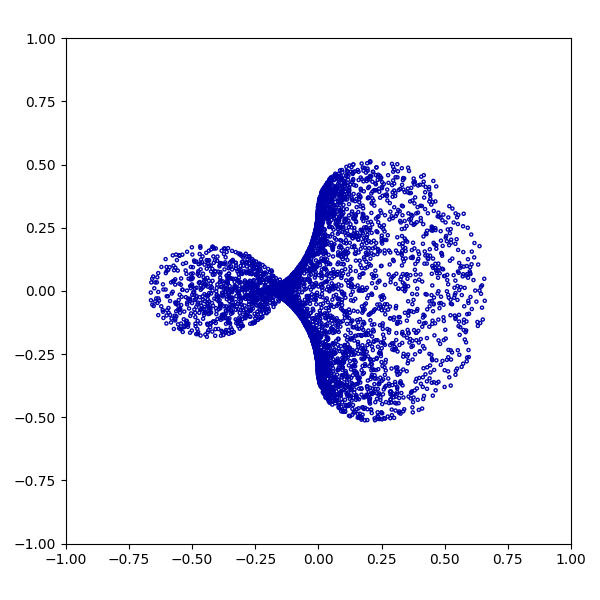
\includegraphics[width=0.1\textwidth]{circle_1_8}
  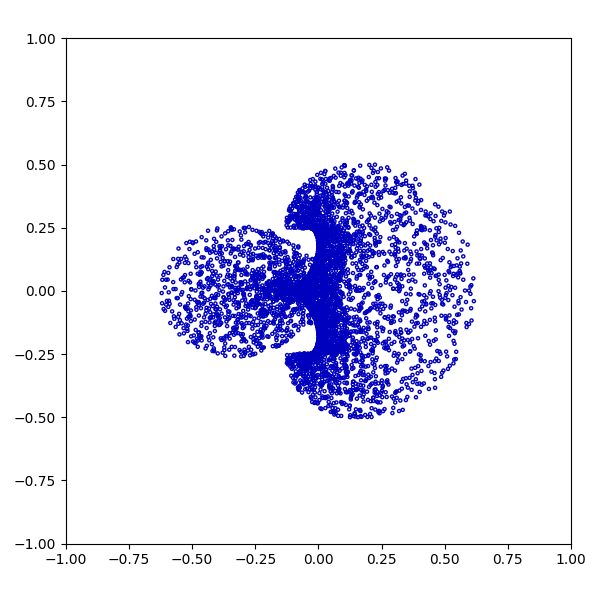
\includegraphics[width=0.1\textwidth]{circle_1_81}
  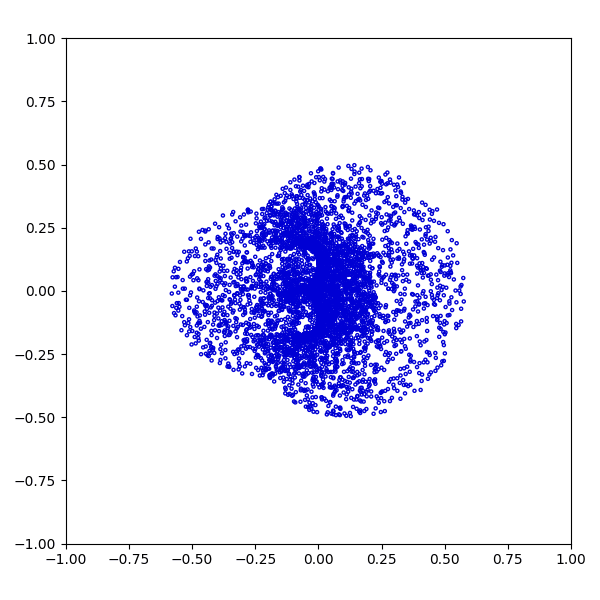
\includegraphics[width=0.1\textwidth]{circle_1_9}
  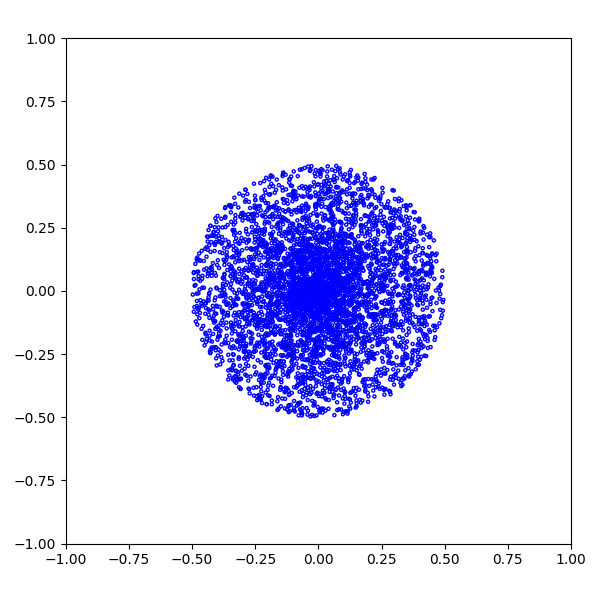
\includegraphics[width=0.1\textwidth]{circle_1_10}
  \caption{从左上到右下可以看出我们的变换$f$如何从Unif$[-1,1]^2$生成所需分布$\mathcal U$}
\end{figure}

\begin{figure}[htbp]
  \centering
  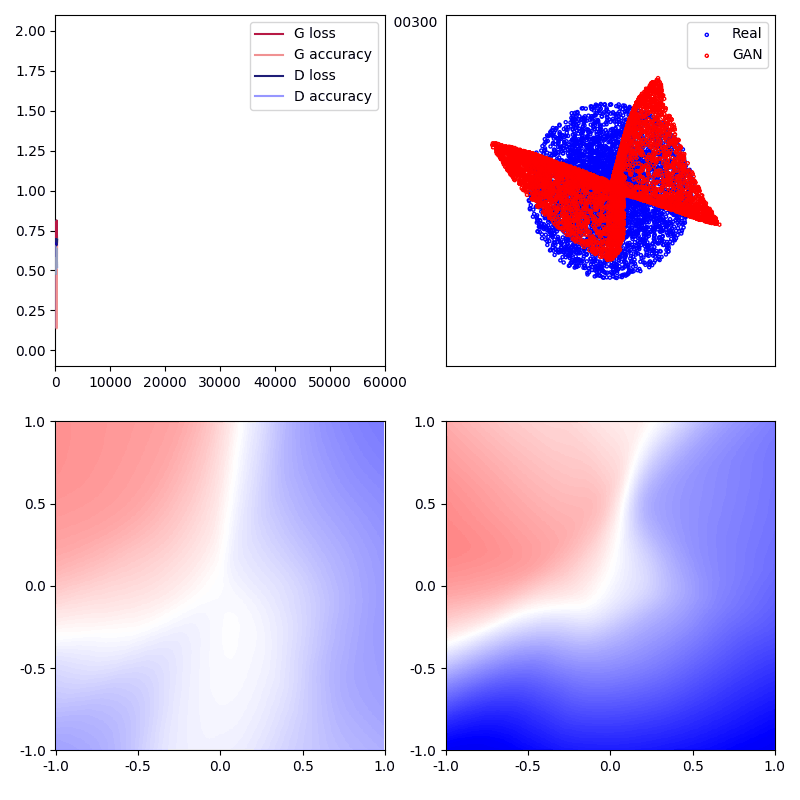
\includegraphics[width=0.3\textwidth]{circle_2_1}
  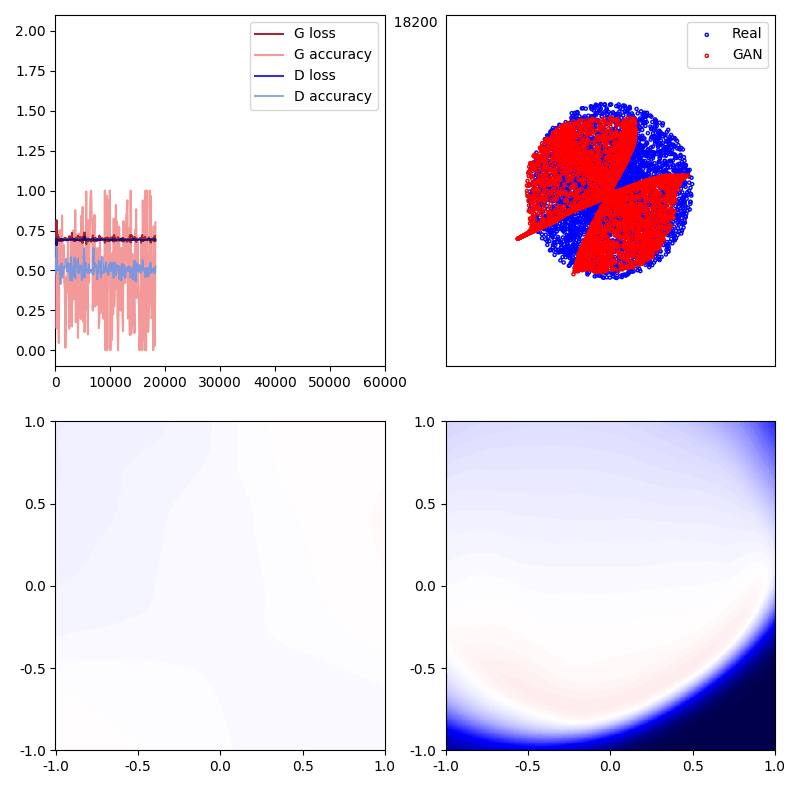
\includegraphics[width=0.3\textwidth]{circle_2_2}\\
  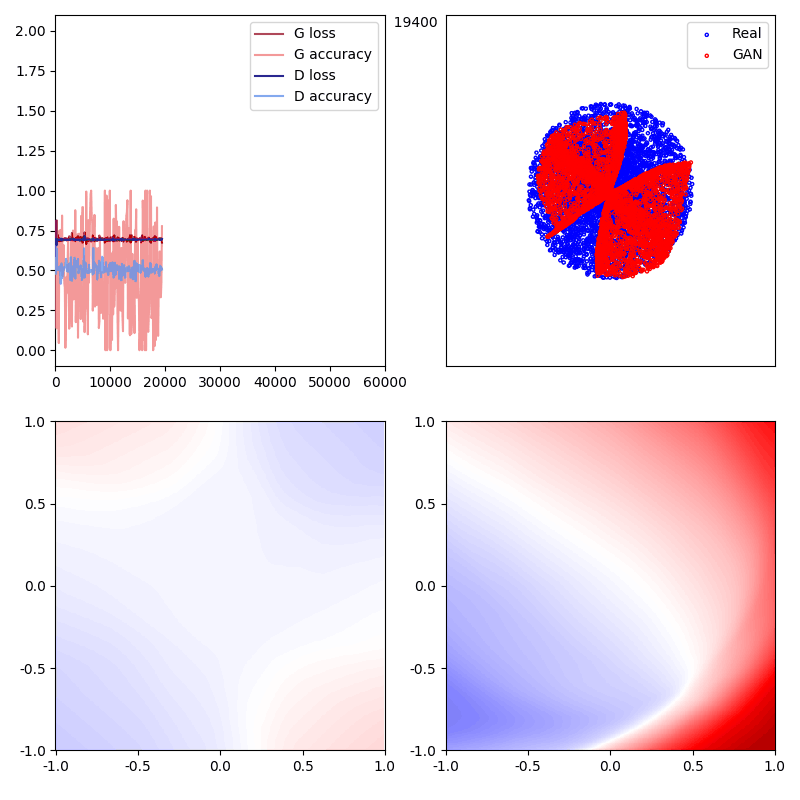
\includegraphics[width=0.3\textwidth]{circle_2_3}
  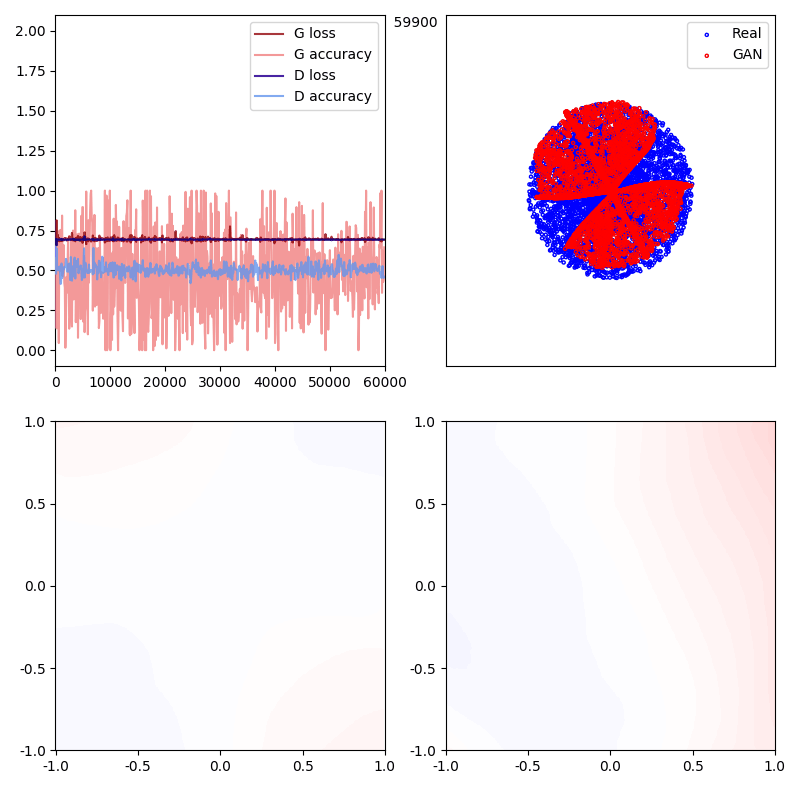
\includegraphics[width=0.3\textwidth]{circle_2_4}
  \caption{\scriptsize 可以看到, 我们的生成器生成的样本并非如我们所想的是圆形, 反而是一个蝴蝶型. 并且之前观察到的判别器的输出在右上与左下之间也观察到了混沌的现象, 其仅相隔一个batch(100个样本), 但判别器却完全推翻之前的结论.}
\end{figure}
可以看到, 生成器并没有像我们想象一样捕捉到圆形分布. 而是捕捉到了分布的大致范围, 以及分布密度从中间到外围逐渐递减的特点. 其生成的样本因为某种未知的原因呈一个蝴蝶型. 并且十分迅速地捕捉到了这个蝴蝶型的分布, 并且在训练的过程中一直保持着这样的蝴蝶型. 

在训练结束的时候判别器基本上处于无效的状态, 对所有的样本都无法给出有效的判断, 自然也无法对生成器进行有效的有意义的引导. 我们还注意到, 在训练的过程中, 判别器的行为有着一定的混沌性. 很多次只间隔一个batch就完全地推翻了之前所给出的结果, 如图中所展示的, 红蓝分布在一个batch的训练后发生了彻底的翻转. 

\subsection{翅膀型}

我们最后一个实验的变换是一个翅膀型的曲线(两个螺线拼接), 即
\begin{align*}
	f_x(x,y) = \dfrac{x}{2} \cos (3x\pi),\ f_y(x,y) = \dfrac{x}{2} \sin (3x\pi).
\end{align*}

\begin{figure}[htpb]
  \centering
  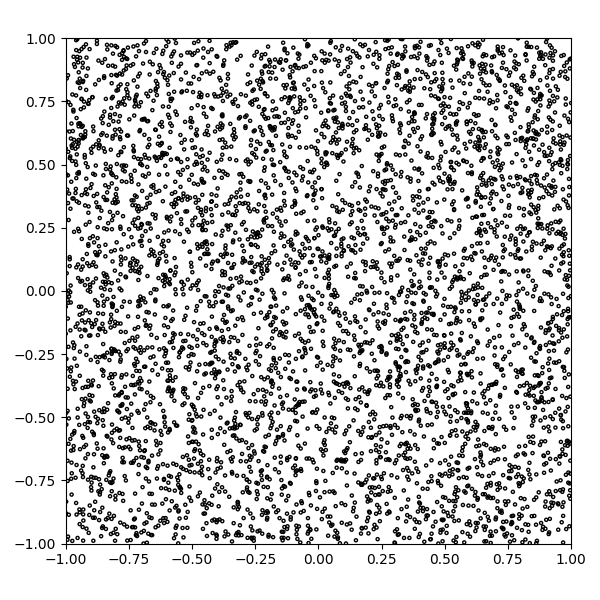
\includegraphics[width=0.15\textwidth]{wings_1_1}
  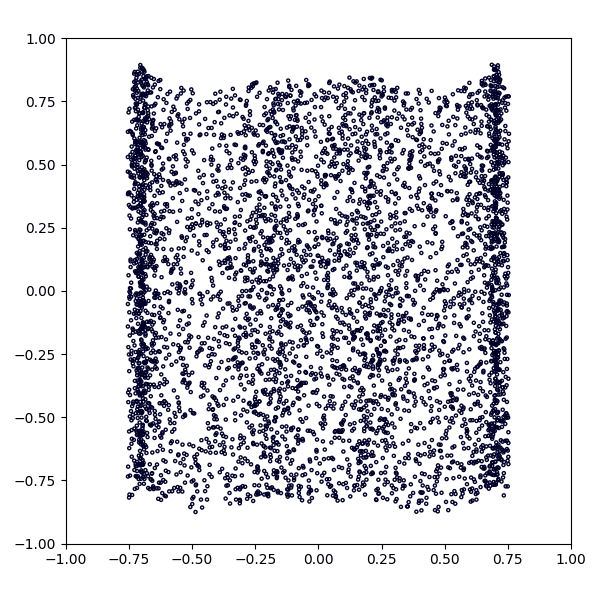
\includegraphics[width=0.15\textwidth]{wings_1_2}
  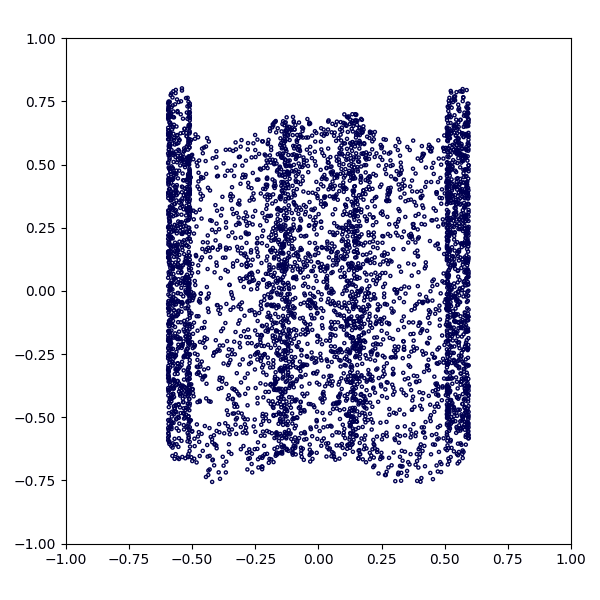
\includegraphics[width=0.15\textwidth]{wings_1_3}
  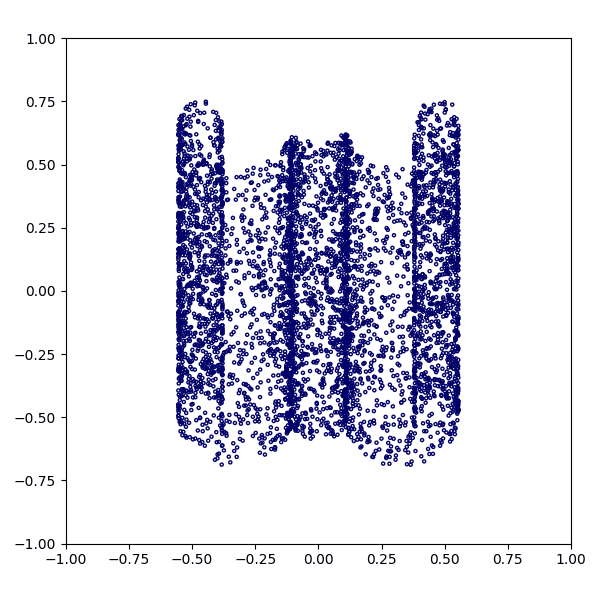
\includegraphics[width=0.15\textwidth]{wings_1_4}
  \includegraphics[width=0.15\textwidth]{wings_1_5}
  \includegraphics[width=0.15\textwidth]{wings_1_6}\\
  \includegraphics[width=0.15\textwidth]{wings_1_7}
  \includegraphics[width=0.15\textwidth]{wings_1_8}
  \includegraphics[width=0.15\textwidth]{wings_1_9}
  \includegraphics[width=0.15\textwidth]{wings_1_10}
  \includegraphics[width=0.15\textwidth]{wings_1_11}
  \includegraphics[width=0.15\textwidth]{wings_1_12}

  
  \caption{从左上到右下可以看出我们的变换$f$如何从Unif$[-1,1]^2$生成所需分布$\mathcal U$}
\end{figure}

这个分布也并非一个均匀分布, 通过变换的过程的可视化以及理论证明都可以得到相同的结果.

\subsubsection{捕捉大致范围}
可以看到, 这次生成器首先捕捉了大概的样本所处的范围. 同时判别器也在捕捉真实样本所处的范围. 并且在输入空间的中下部出现了一个置信度极高的假样本区域(深红色区域), 我们猜测生成器将这部分区域映射到了样本空间的外侧边角. 

\begin{center}
  \includegraphics[width=0.35\textwidth]{wings_2_1}
  \includegraphics[width=0.35\textwidth]{wings_2_2}\\
  \includegraphics[width=0.35\textwidth]{wings_2_3}
  \includegraphics[width=0.35\textwidth]{wings_2_4}
\end{center}

\subsubsection{捕捉分布细节}
可以看到随着训练的进行, 我们的生成器逐渐捕捉到了分布集中在曲线上这一特点. 并且逐渐有更多的点附着到了曲线上. 而判别器这次的表现十分稳固, 在圆内的部分, 真实数据分布在一条曲线上的特征判别器也很好地捕捉到了. 

\begin{figure}[hbp]
  \centering
  \includegraphics[width=0.24\textwidth]{wings_3_1}
  \includegraphics[width=0.24\textwidth]{wings_3_2}
  \includegraphics[width=0.24\textwidth]{wings_3_3}
  \includegraphics[width=0.24\textwidth]{wings_3_4}\\
  \includegraphics[width=0.24\textwidth]{wings_3_5}
  \includegraphics[width=0.24\textwidth]{wings_3_6}
  \includegraphics[width=0.24\textwidth]{wings_3_7}
  \includegraphics[width=0.24\textwidth]{wings_3_8}
  \caption{\scriptsize 可以看到, 在样本空间中逐渐出现了一个高置信的真实样本区域(深蓝色), 这个区域随着训练的进行从左下角出现然后逐渐延伸到两侧, 再逐渐收小最后达到最终结果. 同时随着这个蓝色区域的出现与收缩, 生成器并没有在这两个蓝色区域相应的位置生成样本.}
\end{figure}

有趣的是观察判别器如何随着生成器捕捉到分类边界. 首先一个高置信度的真实样本区间出现在左下角, 随着训练的进行逐渐右下角也出现了这样的一个真实样本区域, 然后两个区域逐渐分离并向上运动, 最后收缩成为两个翅膀的样子. 

与此同时, 生成器在一开始在两个翅膀的位置还是有生成样本的, 但是随着这两个高置信度真实样本区间的出现与收紧, 它就再也没有生成出任何在这两个翅膀的区域上的样本了. 可以说我们的GAN在这个圆里达到了平衡, 但是在翅膀的部分我们的判别器完全支配了生成器. 

同时这时我们再看之前观测到的红色区域, 可以发现, 这个红色区域在此时变成了红色与蓝色交叉的区域, 同时样本空间中的边缘也是红色蓝色相间的. 因此, 基本上可以断定我们的生成器把这个部分映射到了样本空间的边角上.

\section{超参对比}

在这一部分中, 我们用不同的学习率与Adam参数对前面研究过的三个模型再进行了实验, 来探究超参对模型训练的影响. 其中, 圆的训练结果没有任何的改变, 然而正弦波与翅膀型我们通过观察其在不同参数下的表现发现了一些比较有趣的结果. 我们挑选了两组最能说明问题的参数来进行展示.

\subsection{正弦波}

我们将生成器与判别器的优化算法adam的参数$\beta$从$0.5$改到了$0.7$. 可以看到, 网络依旧能够捕捉到大致的分布范围.

\begin{figure}[hbt]
  \centering
  \includegraphics[width=0.22\textwidth]{sin_5_1}
  \includegraphics[width=0.22\textwidth]{sin_5_2}
  \includegraphics[width=0.22\textwidth]{sin_5_3}
  \includegraphics[width=0.22\textwidth]{sin_5_4}\\
  \includegraphics[width=0.22\textwidth]{sin_6_1}
  \includegraphics[width=0.22\textwidth]{sin_6_2}
  \includegraphics[width=0.22\textwidth]{sin_6_3}
  \includegraphics[width=0.22\textwidth]{sin_6_4}
\end{figure}

但在捕捉到了大致范围以后, 却无法捕捉到任何细致的分布. 同时, 还能够观察到在之前的实验中出现的样本集中到对角线上的现象迅速出现. 并且在这个现象出现以后, 网络便几乎停止了更新. 尽管可以明显地看到大部分样本不正确的集中在两个波峰之间的空白区域, 但是判别器已经无法指导我们的生成器进行更新了. 所以我们猜测之前所观察到的现象是陷入到了一个局部的极小值中. GAN在陷入了之后无法自己通过更新参数逃出这个陷阱. 

\subsection{翅膀型}

我们选择了一组新的参数, 生成器的学习率为0.0005, Adam参数为$\beta=0.9$. 判别器的学习率为0.05, Adam参数为$\beta=0.9$. 在这样的参数设定下, 生成器甚至无法捕捉到初始的分布的轮廓. 其生成的数据缩小成了一小块区域, 围绕真实数据进行震荡, 随着训练的进行这样的震荡更多地集中在了数据中心.

\begin{figure}[hbt]
\centering
  \includegraphics[width=0.35\textwidth]{wings_4_1}
  \includegraphics[width=0.35\textwidth]{wings_4_2}\\
  \includegraphics[width=0.35\textwidth]{wings_4_3}
  \includegraphics[width=0.35\textwidth]{wings_4_4}
\end{figure}

但是尽管如此一直到600个batch以后, 我们的网络依旧还是处在一个无法捕捉大致范围的阶段.

\section{总结}

我们对于生成式对抗网络进行了实际的动手训练, 训练了一个简单的图像生成器, 虽然受限于计算资源与有限的精力, 无法将结果调整至以假乱真的境界, 但是在这其中我们也可以看出训练生成式对抗网络所需要的启发性技巧的必要性. 

进一步, 我们对生成式对抗网络的训练过程进行了可视化, 揭示了在一个更简单的问题上生成器与判别器是如何一起学习生成我们期望的分布的. 它首先通过不断尝试来捕捉大致的分布范围, 然后再在细节上进行优化. 接着我们还观察到了在收敛以后网络竟然能够随着训练的深入陷入到局部极小值中. 并且从这个现象出发进一步进行了实验, 研究了超参的设置如何影响训练过程. 发现不同的超参可能在我们前面确定的训练的不同阶段有着不同的影响. 最后通过对不同超参的实验结果, 推测是因为超参数的设置导致了之前的网络在收敛以后又进一步陷入局部极小值的情况. 

生成式对抗网络无疑是一种极具启发式的网络架构. 但是通过这次实验, 我们有一个疑问, 即这种无监督架构真的是“无监督”的吗? 其对超参数调整所需要的人力和时间成本, 以及在调参与训练过程中对计算资源的要求使得这样的无监督学习很难真的令人相信它真的是“无监督”的. 与其说是GAN是一种“无监督”模型, 倒不如说它是当今的“土豪模型”的代表之一. 

倘若没有极度充足的经费、相当大规模的计算机集群, 进入到前沿的GAN的研究中去是几乎不可能的事情. 机器学习的竞争变成了先是计算资源的竞争, 之后才是智慧的竞争. 并且这样的“无监督”对超参数调整的需求更加体现出了元学习的重要性, 因此, 从这样的“无监督”到真正的无监督, 我们还差一步 \textcolor{red}{Learning to Learn}.


\newpage
\nocite{*}

\bibliographystyle{unsrt}
\bibliography{wpref}

\end{document}
